% BEGIN AUTO-GENERATED APPENDIX EXPERIMENT RESULTS
% This file is generated by experiments/export_appendix_report.py.
% Do not edit table values by hand; regenerate them from the result summaries.
\section{论文附录部分实验复现}
\label{sec:appendix-reproduction}

\subsection{实验协议与统计口径}
我们复现了原论文附录 B 中的五类分类任务,代码选取的重上传层数为
$\{1,2,3,4,5,6,8,10\}$，共 8 种。
对于普通保真度损失 $\chi_f^2$，实验包含
1 量子比特无纠缠、2 量子比特无纠缠和 2 量子比特有纠缠三类电路；
前两类各有 8 种层数，而有纠缠电路只有 7 种，因为代码中的 CZ 门只插入相邻重上传层之间，
当层数为 1 时不存在可插入纠缠门的位置，故共有
$8+8+7=23$ 组。
对于加权保真度损失 $\chi_{wf}^2$，除上述 23 组外，还加入
4 量子比特无纠缠的 8 组和 4 量子比特有纠缠的 7 组，故共有
$23+8+7=38$ 组。
因此每个任务的实验总数为 $23+38=61$，共 305 实验。

4 量子比特实验中只使用 $\chi_{wf}^2$：
普通保真度代码令标签态量子比特数等于分类器量子比特数，并直接计算完整输出态与全局标签态的保真度，
但当前 \texttt{representatives} 函数只实现了 1 和 2 量子比特标签态，没有实现 4 量子比特标签态；
若直接运行 4 量子比特的 $\chi_f^2$，会得到未定义的全零标签向量。
相比之下，加权保真度固定使用单量子比特标签态，先从每个物理量子比特的约化密度矩阵计算局部保真度，
再通过可训练权重将各量子比特的结果组合起来，因此可以直接推广到 4 量子比特。
这属于当前代码实现和论文复现实验网格的限制，并不意味着普通保真度在理论上不能用于 4 量子比特分类器。

其中二维任务使用 200 个训练点和 4000 个测试点, 三维球任务使用 500 个训练点和 4000 个测试点; 优化器均为 L-BFGS-B. 每个配置只使用随机种子 30 训练一次。

\begin{table}[H]
    \centering
    \caption{五类任务的最佳配置及固定测试集 Wilson 区间}
    \label{tab:appendix-best-summary}
    \small
    \begin{tabular}{lcccccc}
        \toprule
        任务       & 最高准确率   & 损失            & 比特数 & 纠缠 & 层数 \\
        \midrule
        非凸边界问题   & 97.75\% & $\chi_{wf}^2$ & 2   & 无  & 8  \\
        二分类圆环问题  & 97.25\% & $\chi_{wf}^2$ & 2   & 无  & 5  \\
        三维球问题    & 96.17\% & $\chi_{wf}^2$ & 4   & 有  & 2  \\
        四分类方块问题  & 98.58\% & $\chi_f^2$    & 2   & 有  & 5  \\
        四分类波浪线问题 & 93.90\% & $\chi_{wf}^2$ & 4   & 有  & 8  \\
        \bottomrule
    \end{tabular}
\end{table}

\subsection{完整准确率网格}
表~\ref{tab:appendix-all-results} 给出全部 305 组准确率. 非凸边界任务由 $x_2=-2x_1+1.5\sin(\pi x_1)$ 划分类别; 圆环任务要求识别两个同心圆之间的不连通区域; 三维球任务检验三维输入编码; 方块任务是四象限线性边界; 波浪线任务同时包含四分类、非凸边界和面积较小的局部区域. 一层电路未插入 CZ 门.

\begin{table}[htbp]
    \centering
    \scriptsize
    \caption{不同测试问题的模型准确率对比}
    \label{tab:appendix-all-results}
    \setlength{\tabcolsep}{4pt}
    \renewcommand{\arraystretch}{0.85}
    \begin{tabular}{c*{8}{c}}
        \toprule
        \multirow{2}{*}{层数} & \multicolumn{3}{c}{$\chi_f^2$} & \multicolumn{5}{c}{$\chi_{wf}^2$}                                           \\
        \cmidrule(lr){2-4}\cmidrule(lr){5-9}
                            & 1q                             & \shortstack{2q                                                              \\无纠缠} & \shortstack{2q\\有纠缠}
                            & 1q                             & \shortstack{2q                                                              \\无纠缠} & \shortstack{2q\\有纠缠}
                            & \shortstack{4q                                                                                               \\无纠缠} & \shortstack{4q\\有纠缠} \\
        \midrule
        \multicolumn{9}{c}{\textbf{(a) 非凸边界问题}}                                                                                            \\
        \midrule
        1                   & 0.49                           & 0.55                              & --   & 0.49 & 0.76 & --   & 0.76 & --   \\
        2                   & 0.82                           & 0.75                              & 0.75 & 0.86 & 0.95 & 0.85 & 0.96 & 0.96 \\
        3                   & 0.89                           & 0.74                              & 0.85 & 0.95 & 0.95 & 0.95 & 0.95 & 0.97 \\
        4                   & 0.75                           & 0.74                              & 0.88 & 0.95 & 0.95 & 0.97 & 0.95 & 0.97 \\
        5                   & 0.95                           & 0.95                              & 0.90 & 0.94 & 0.95 & 0.97 & 0.95 & 0.97 \\
        6                   & 0.95                           & 0.94                              & 0.93 & 0.97 & 0.96 & 0.97 & 0.95 & 0.97 \\
        8                   & 0.95                           & 0.96                              & 0.95 & 0.97 & 0.98 & 0.97 & 0.96 & 0.97 \\
        10                  & 0.95                           & 0.93                              & 0.95 & 0.96 & 0.96 & 0.96 & 0.96 & 0.97 \\

        \midrule
        \multicolumn{9}{c}{\textbf{(b) 二分类圆环问题}}                                                                                           \\
        \midrule
        1                   & 0.44                           & 0.50                              & --   & 0.44 & 0.57 & --   & 0.66 & --   \\
        2                   & 0.48                           & 0.50                              & 0.51 & 0.53 & 0.72 & 0.71 & 0.70 & 0.96 \\
        3                   & 0.49                           & 0.50                              & 0.56 & 0.74 & 0.78 & 0.96 & 0.76 & 0.97 \\
        4                   & 0.81                           & 0.69                              & 0.56 & 0.86 & 0.97 & 0.97 & 0.92 & 0.96 \\
        5                   & 0.88                           & 0.91                              & 0.88 & 0.83 & 0.97 & 0.95 & 0.97 & 0.95 \\
        6                   & 0.90                           & 0.93                              & 0.93 & 0.93 & 0.94 & 0.95 & 0.95 & 0.93 \\
        8                   & 0.91                           & 0.93                              & 0.94 & 0.93 & 0.94 & 0.93 & 0.96 & 0.94 \\
        10                  & 0.90                           & 0.92                              & 0.91 & 0.92 & 0.95 & 0.93 & 0.96 & 0.93 \\

        \midrule
        \multicolumn{9}{c}{\textbf{(c) 三维球问题}}                                                                                             \\
        \midrule
        1                   & 0.53                           & 0.70                              & --   & 0.53 & 0.70 & --   & 0.70 & --   \\
        2                   & 0.77                           & 0.73                              & 0.53 & 0.78 & 0.94 & 0.96 & 0.96 & 0.96 \\
        3                   & 0.76                           & 0.74                              & 0.77 & 0.78 & 0.92 & 0.94 & 0.95 & 0.95 \\
        4                   & 0.84                           & 0.79                              & 0.77 & 0.89 & 0.92 & 0.95 & 0.95 & 0.94 \\
        5                   & 0.87                           & 0.85                              & 0.77 & 0.90 & 0.94 & 0.94 & 0.94 & 0.94 \\
        6                   & 0.90                           & 0.87                              & 0.88 & 0.92 & 0.94 & 0.93 & 0.93 & 0.94 \\
        8                   & 0.89                           & 0.88                              & 0.90 & 0.94 & 0.91 & 0.94 & 0.94 & 0.93 \\
        10                  & 0.93                           & 0.91                              & 0.90 & 0.93 & 0.94 & 0.92 & 0.92 & 0.92 \\

        \midrule
        \multicolumn{9}{c}{\textbf{(d) 四分类方块问题}}                                                                                           \\
        \midrule
        1                   & 0.58                           & 0.48                              & --   & 0.71 & 0.92 & --   & 0.90 & --   \\
        2                   & 0.76                           & 0.96                              & 0.96 & 0.74 & 0.91 & 0.94 & 0.94 & 0.95 \\
        3                   & 0.90                           & 0.93                              & 0.98 & 0.90 & 0.94 & 0.95 & 0.95 & 0.95 \\
        4                   & 0.89                           & 0.98                              & 0.95 & 0.88 & 0.95 & 0.95 & 0.95 & 0.95 \\
        5                   & 0.91                           & 0.98                              & 0.99 & 0.89 & 0.94 & 0.94 & 0.95 & 0.94 \\
        6                   & 0.92                           & 0.98                              & 0.94 & 0.93 & 0.94 & 0.95 & 0.94 & 0.94 \\
        8                   & 0.94                           & 0.98                              & 0.94 & 0.93 & 0.94 & 0.95 & 0.95 & 0.94 \\
        10                  & 0.95                           & 0.97                              & 0.93 & 0.94 & 0.93 & 0.94 & 0.94 & 0.93 \\

        \midrule
        \multicolumn{9}{c}{\textbf{(e) 四分类波浪线问题}}                                                                                          \\
        \midrule
        1                   & 0.70                           & 0.52                              & --   & 0.76 & 0.75 & --   & 0.89 & --   \\
        2                   & 0.86                           & 0.75                              & 0.80 & 0.84 & 0.89 & 0.88 & 0.91 & 0.92 \\
        3                   & 0.74                           & 0.85                              & 0.84 & 0.84 & 0.92 & 0.91 & 0.92 & 0.91 \\
        4                   & 0.80                           & 0.85                              & 0.87 & 0.87 & 0.90 & 0.93 & 0.92 & 0.93 \\
        5                   & 0.85                           & 0.90                              & 0.88 & 0.87 & 0.92 & 0.93 & 0.93 & 0.93 \\
        6                   & 0.92                           & 0.92                              & 0.91 & 0.86 & 0.93 & 0.94 & 0.93 & 0.93 \\
        8                   & 0.89                           & 0.91                              & 0.91 & 0.92 & 0.93 & 0.93 & 0.93 & 0.94 \\
        10                  & 0.92                           & 0.91                              & 0.93 & 0.90 & 0.93 & 0.93 & 0.93 & 0.93 \\
        \bottomrule
    \end{tabular}
\end{table}

\subsection{层数效应与饱和区间}
图~\ref{fig:appendix-layer-trends} (a)左图只比较普通与加权损失共同拥有的1q、2q 无纠缠和 2q 有纠缠配置, 在这些架构上,统计平均值 普通保真度平均准确率从一层的 55.01\%上升到十层的 92.63\%, 加权保真度则从 66.25\% 上升到 93.56\%. (a)右图统计相同层数所有架构,  达到 90\% 的比例从一层的 4\% 增至五层的70\%, 六层和八层均为 90\%, 十层为 95\%. 与此同时, 全配置平均准确率在五、六、八、十层分别为 91.98\%、93.27\%、93.56\% 和 93.28\%, 这在一定程度上可以说明主要增益集中在前五至六层, 此后总体进入平台区.

\begin{figure}[htbp]
    \centering
    \begin{subfigure}[t]{0.57\textwidth}
        \centering
        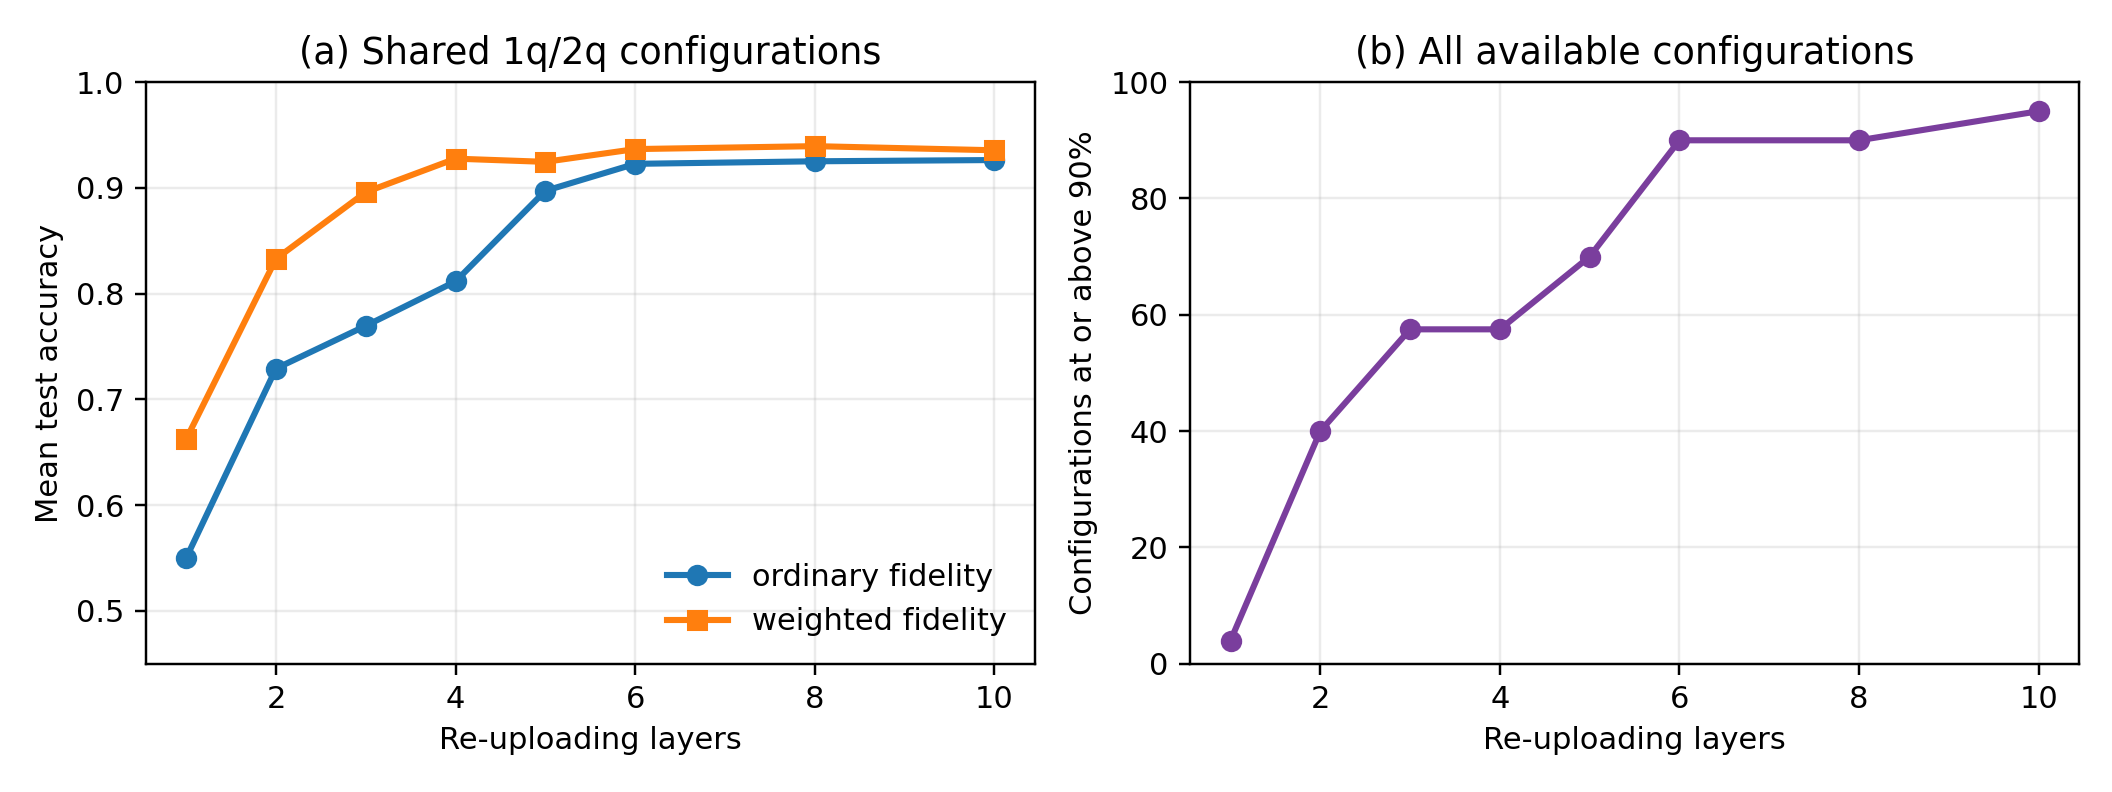
\includegraphics[width=\linewidth]{figures/appendix_results/layer_trends.png}
        \caption{架构平均准确率与达到 90\% 的配置比例}
    \end{subfigure}
    \hfill
    \begin{subfigure}[t]{0.40\textwidth}
        \centering
        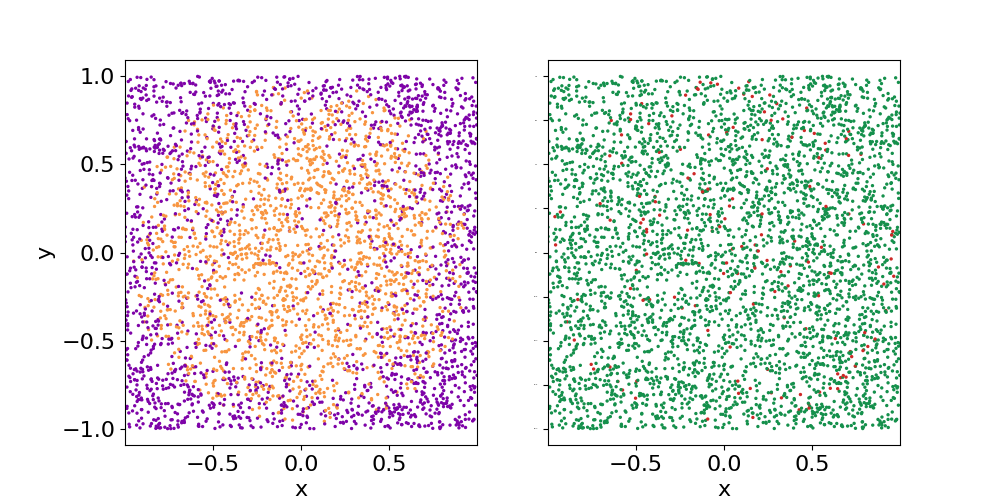
\includegraphics[width=\linewidth]{figures/appendix_results/sphere_best.png}
        \caption{三维球最佳模型的 $xy$ 投影, 准确率 96.17\%}
    \end{subfigure}
    \caption{层数总体趋势与此前未展示的三维球结果}
    \label{fig:appendix-layer-trends}
\end{figure}

此外,统计还得出, 40 条层数序列中有 38 条至少出现一次随层数增加而下降; 全部 265 个相邻层数转换中有 100 个下降, 最大单步下降为 14.75 个百分点. 最大下降实例出现在非凸边界问题的 $\chi_f^2$、1q、无纠缠架构: 从 3 层的 89.33\% 降至 4 层的 74.58\%. 图~\ref{fig:appendix-worst-depth-drop} 显示, 较深模型并非缺少表达该边界的能力, 而是本次独立优化得到的决策区域退化为近似水平分割, 在正弦边界的弯曲区域产生大量错误. 因而“更深通常更好”只在总体平均意义上成立, 不能作为单个训练实例的单调性结论. 该现象与非凸优化陷入较差局部极小值相符, 但仅凭单随机种子仍不能把下降唯一归因于局部极小值; 还需要多随机种子和优化轨迹验证.

\begin{figure}[htbp]
    \centering
    \begin{subfigure}[t]{0.48\textwidth}
        \centering
        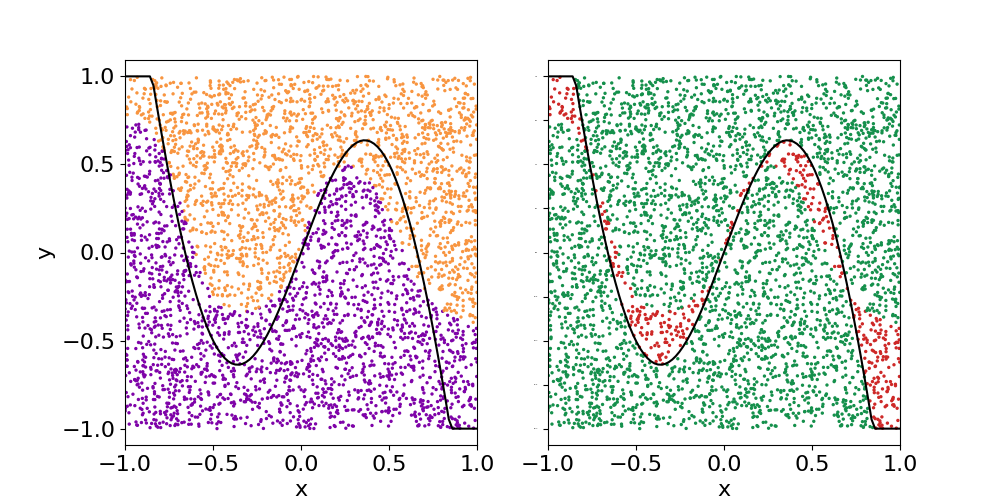
\includegraphics[width=\linewidth]{figures/appendix_results/worst_depth_drop_before.png}
        \caption{3 层: 89.33\%}
    \end{subfigure}
    \hfill
    \begin{subfigure}[t]{0.48\textwidth}
        \centering
        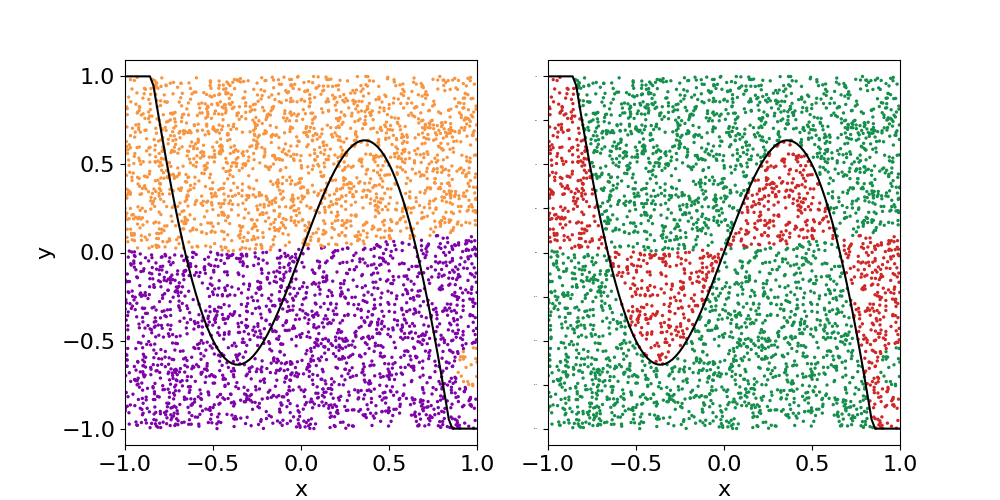
\includegraphics[width=\linewidth]{figures/appendix_results/worst_depth_drop_after.png}
        \caption{4 层: 74.58\%}
    \end{subfigure}
    \caption{最大相邻层数下降实例: 非凸边界问题, $\chi_f^2$, 1q, 无纠缠; 增加一层后下降 14.75 个百分点}
    \label{fig:appendix-worst-depth-drop}
\end{figure}

\begin{figure}[htbp]
    \centering
    \begin{subfigure}[t]{0.32\textwidth}
        \centering
        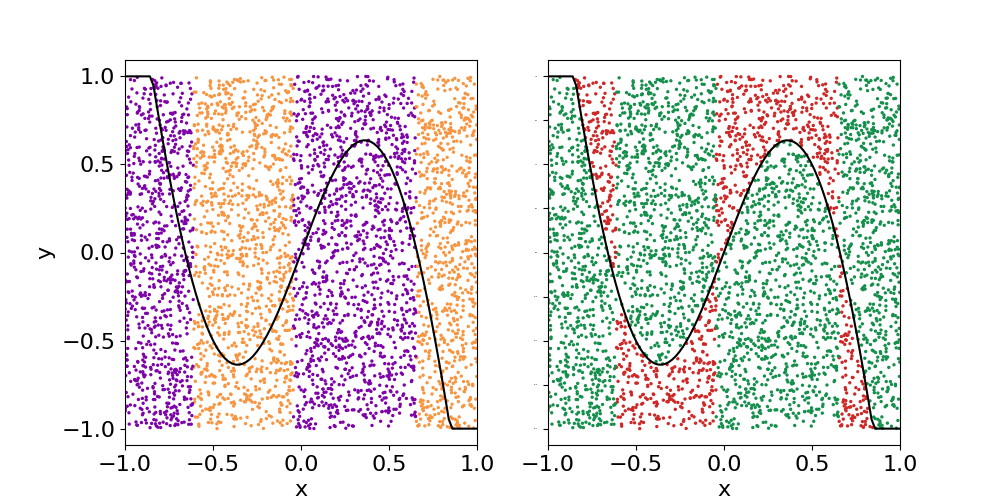
\includegraphics[width=\linewidth]{figures/appendix_results/nonconv_depth_l1.png}
        \caption{1 层: 75.58\%}
    \end{subfigure}
    \hfill
    \begin{subfigure}[t]{0.32\textwidth}
        \centering
        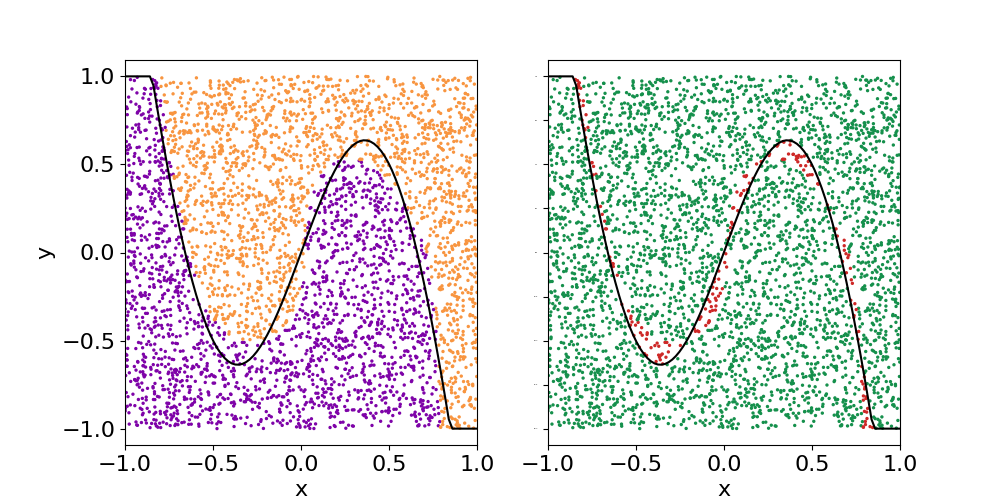
\includegraphics[width=\linewidth]{figures/appendix_results/nonconv_depth_l3.png}
        \caption{3 层: 94.93\%}
    \end{subfigure}
    \hfill
    \begin{subfigure}[t]{0.32\textwidth}
        \centering
        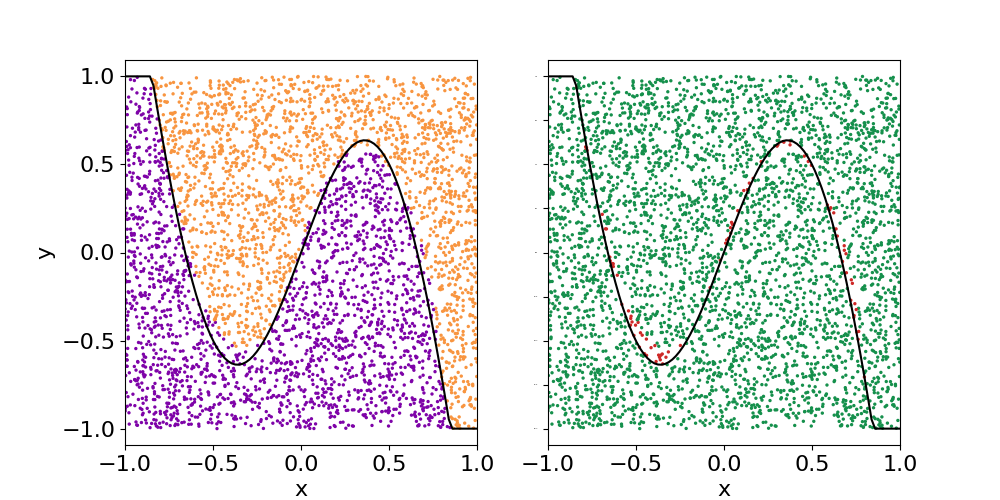
\includegraphics[width=\linewidth]{figures/appendix_results/nonconv_depth_l8.png}
        \caption{8 层: 97.75\%}
    \end{subfigure}
    \caption{同一 $\chi_{wf}^2$、2q 无纠缠架构随重上传层数增加的决策区域}
    \label{fig:appendix-depth-progression}
\end{figure}

\subsection{损失函数的配对比较}
为避免 4q 配置只存在于加权损失一侧造成结构混杂, 表~\ref{tab:appendix-objective-pairs} 仅在相同任务、比特数、层数和纠缠设置下比较两种损失, 每个任务含 23 对, 总计 115 对. 加权保真度的平均增益为 6.34 个百分点, 中位增益为 2.45 个百分点, 并在 92/115 个配对中占优. 但方块任务的平均增益只有 0.77 个百分点, 且仅 8/23 个配对占优, 说明加权损失并非对所有几何边界都稳定更好.

\begin{table}[htbp]
    \centering
    \caption{共享架构上加权保真度相对普通保真度的配对差值}
    \label{tab:appendix-objective-pairs}
    \small
    \begin{tabular}{lrrrr}
        \toprule
        任务       & 平均差值/百分点 & 中位差值/百分点 & 加权胜出   & 普通胜出   \\
        \midrule
        非凸边界问题   & +7.29    & +3.48    & 21/23  & 2/23   \\
        二分类圆环问题  & +10.50   & +4.60    & 21/23  & 2/23   \\
        三维球问题    & +8.67    & +4.57    & 23/23  & 0/23   \\
        四分类方块问题  & +0.77    & -1.28    & 8/23   & 15/23  \\
        四分类波浪线问题 & +4.46    & +2.50    & 19/23  & 4/23   \\
        总体       & +6.34    & +2.45    & 92/115 & 23/115 \\
        \bottomrule
    \end{tabular}
\end{table}

\begin{figure}[htbp]
    \centering
    \begin{subfigure}[t]{0.48\textwidth}
        \centering
        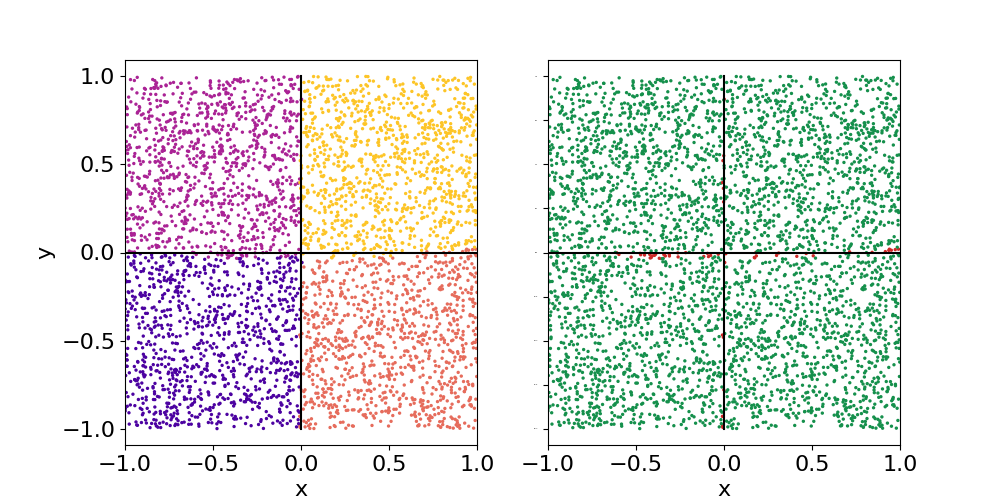
\includegraphics[width=\linewidth]{figures/appendix_results/squares_l5_ordinary.png}
        \caption{$\chi_f^2$: 98.58\%}
    \end{subfigure}
    \hfill
    \begin{subfigure}[t]{0.48\textwidth}
        \centering
        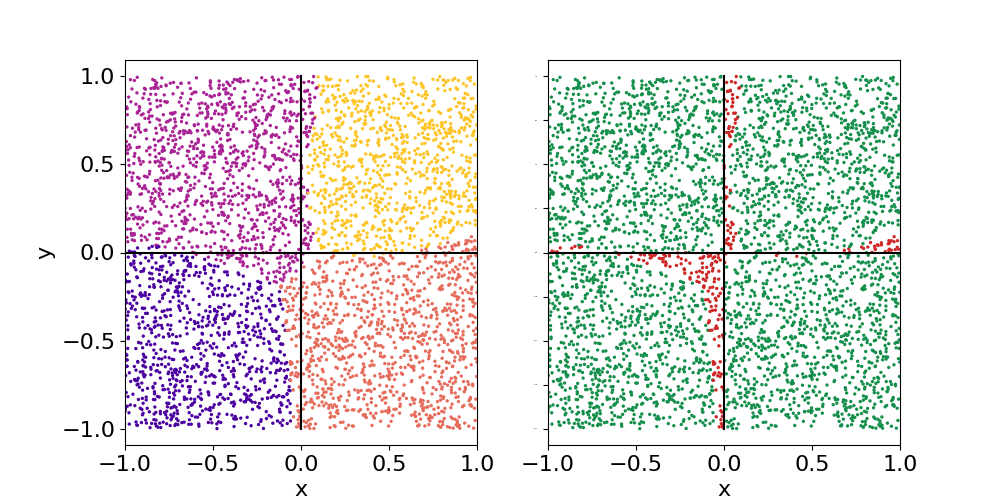
\includegraphics[width=\linewidth]{figures/appendix_results/squares_l5_weighted.png}
        \caption{$\chi_{wf}^2$: 93.60\%}
    \end{subfigure}
    \caption{方块任务中同为 2q、有纠缠、5 层时两种损失的结果对照}
    \label{fig:appendix-loss-comparison}
\end{figure}

\subsection{纠缠效应的异质性}
在固定任务、损失、比特数和层数后, 共得到 105 对有纠缠与无纠缠结果. 有纠缠模型平均只提高 0.53 个百分点, 中位数为 0.25 个百分点; 59 对提高, 46 对下降, 差值范围为 -20.60 至 25.55 个百分点. 因此不能仅凭平均值断言纠缠必然改善分类. 图~\ref{fig:appendix-entanglement-comparison} 展示收益最大的圆环实例: 4q、2 层加权模型加入 CZ 后由 70.45\% 提升至 96.00\%, 说明纠缠的价值主要取决于任务结构与当前深度.

\begin{figure}[H]
    \centering
    \begin{subfigure}[t]{0.48\textwidth}
        \centering
        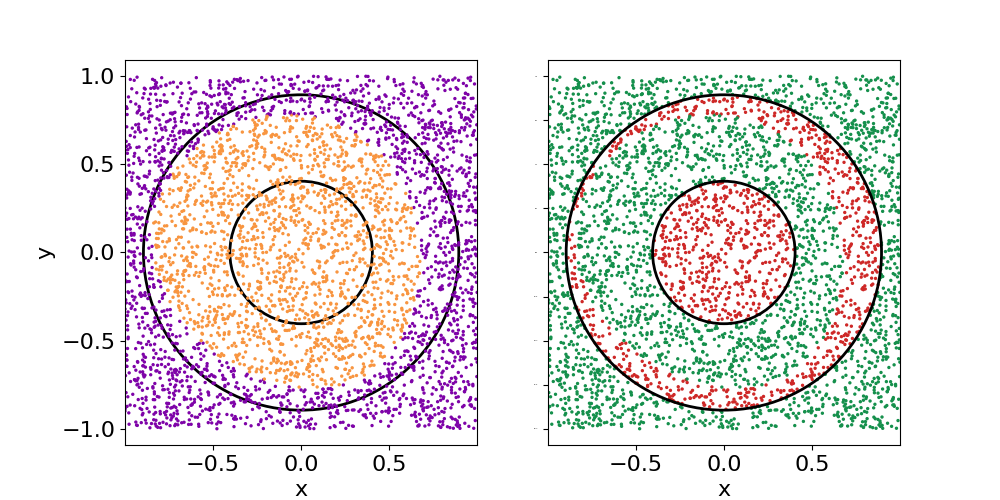
\includegraphics[width=\linewidth]{figures/appendix_results/crown_4q_l2_separable.png}
        \caption{无纠缠: 70.45\%}
    \end{subfigure}
    \hfill
    \begin{subfigure}[t]{0.48\textwidth}
        \centering
        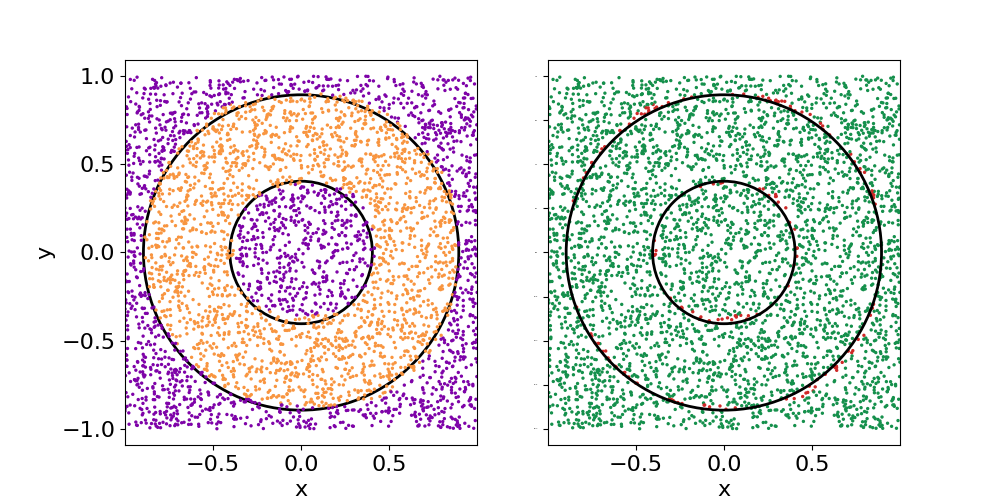
\includegraphics[width=\linewidth]{figures/appendix_results/crown_4q_l2_entangled.png}
        \caption{有纠缠: 96.00\%}
    \end{subfigure}
    \caption{圆环任务中同为 $\chi_{wf}^2$、4q、2 层时的纠缠对照}
    \label{fig:appendix-entanglement-comparison}
\end{figure}

\subsection{各二维任务的最佳决策区域}
图~\ref{fig:appendix-best-results} 汇总四个二维任务的最佳结果. 每幅图左侧为预测类别, 右侧以绿色和红色标记正确与错误测试点. 这些图用于展示最佳可达边界, 而图~\ref{fig:appendix-depth-progression}--\ref{fig:appendix-entanglement-comparison} 则补充了原论文未集中展示的深度、损失与纠缠对照.

\begin{figure}[htbp]
    \centering
    \begin{subfigure}[t]{0.48\textwidth}
        \centering
        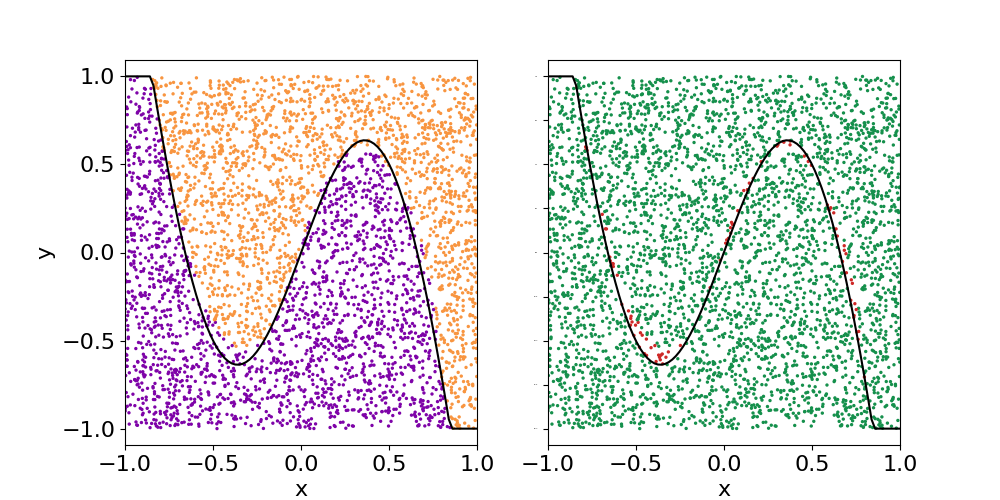
\includegraphics[width=\linewidth]{figures/appendix_results/non_convex.png}
        \caption{非凸边界问题: $\chi_{wf}^2$, 2 量子比特, 无纠缠, 8 层, 准确率 97.75\%}
        \label{fig:appendix-non_convex-best}
    \end{subfigure}
    \hfill
    \begin{subfigure}[t]{0.48\textwidth}
        \centering
        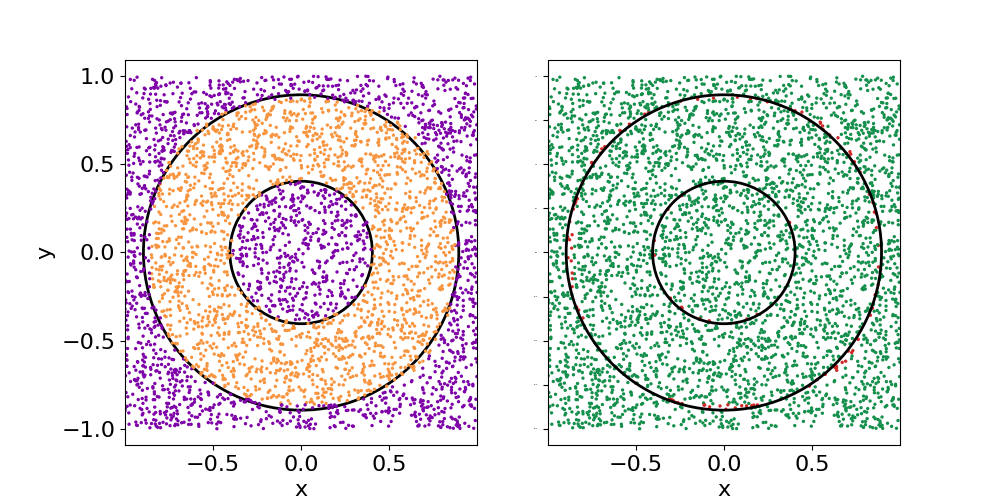
\includegraphics[width=\linewidth]{figures/appendix_results/crown.png}
        \caption{二分类圆环问题: $\chi_{wf}^2$, 2 量子比特, 无纠缠, 5 层, 准确率 97.25\%}
        \label{fig:appendix-crown-best}
    \end{subfigure}
    \par\medskip
    \begin{subfigure}[t]{0.48\textwidth}
        \centering
        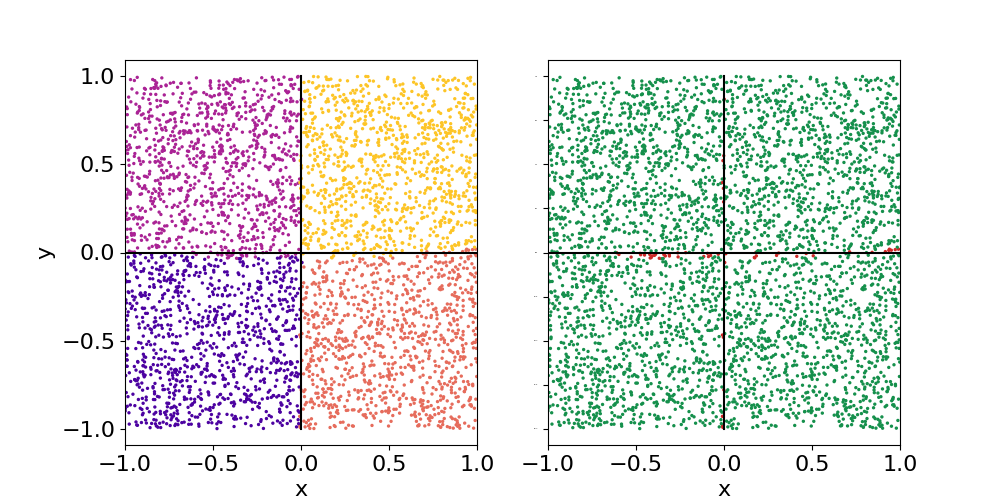
\includegraphics[width=\linewidth]{figures/appendix_results/squares.png}
        \caption{四分类方块问题: $\chi_f^2$, 2 量子比特, 有纠缠, 5 层, 准确率 98.58\%}
        \label{fig:appendix-squares-best}
    \end{subfigure}
    \hfill
    \begin{subfigure}[t]{0.48\textwidth}
        \centering
        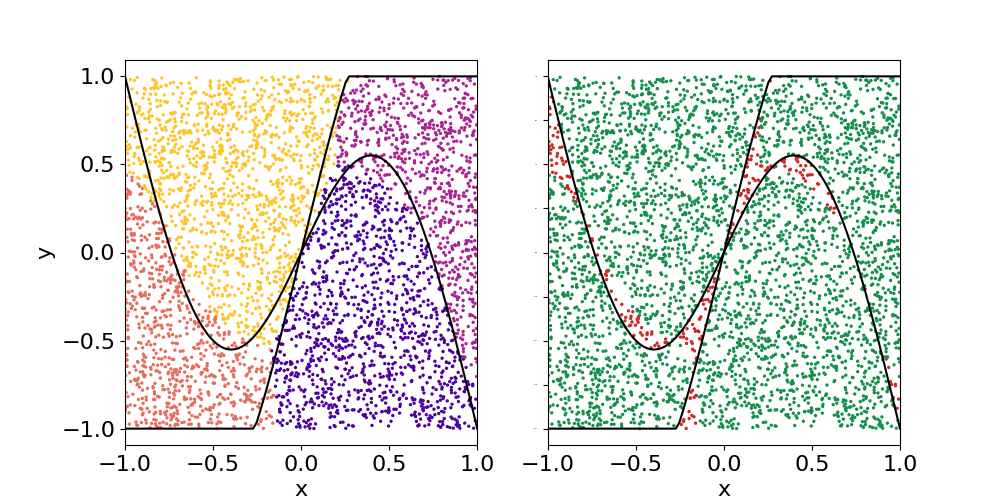
\includegraphics[width=\linewidth]{figures/appendix_results/wavy_lines.png}
        \caption{四分类波浪线问题: $\chi_{wf}^2$, 4 量子比特, 有纠缠, 8 层, 准确率 93.90\%}
        \label{fig:appendix-wavy_lines-best}
    \end{subfigure}
    \par\medskip
    \caption{附录四个二维任务的最佳复现实验结果}
    \label{fig:appendix-best-results}
\end{figure}

\enlargethispage{2\baselineskip}
\subsection{结论与限制}
305 组结果支持三个有限结论. 第一, 重上传层数是最稳定的容量来源, 平均性能在五至六层后趋于饱和, 但单次训练结果高度非单调. 第二, 在严格匹配的共享架构上, 加权保真度总体优于普通保真度, 但优势在方块任务上明显减弱, 最佳方块模型反而来自普通保真度. 第三, 纠缠的总体平均收益很小且正负并存, 其作用更接近任务相关的表达能力补充, 而不是普遍增益. 以上结果均来自单一训练种子; 若要作统计推断, 仍需对每个配置使用多个独立初始化, 报告均值、标准差或置信区间, 并对同一测试集上的配对差值采用配对重采样或 McNemar 检验.
% END AUTO-GENERATED APPENDIX EXPERIMENT RESULTS

\clearpage
